\chapter{Metodologia}
% Nesta seção, serão definidas as métricas específicas que serão utilizadas para avaliar a eficácia dos processamentos de imagem no estudo.

A metodologia delineada neste estudo tem como propósito fundamental o desenvolvimento de um arcabouço sistemático para aprimorar, comparar, selecionar e combinar técnicas de processamento de imagem, visando aprimorar a detecção e classificação de falhas em cadeias de isoladores. O processo é estruturado e iterativo, conforme ilustrado no fluxograma da Figura \ref{fig:fluxograma_metodologia}.

\begin{figure}[H]
    \centering
    \caption{\label{fig:fluxograma_metodologia}Fluxograma da metodologia de processamento de imagens}
    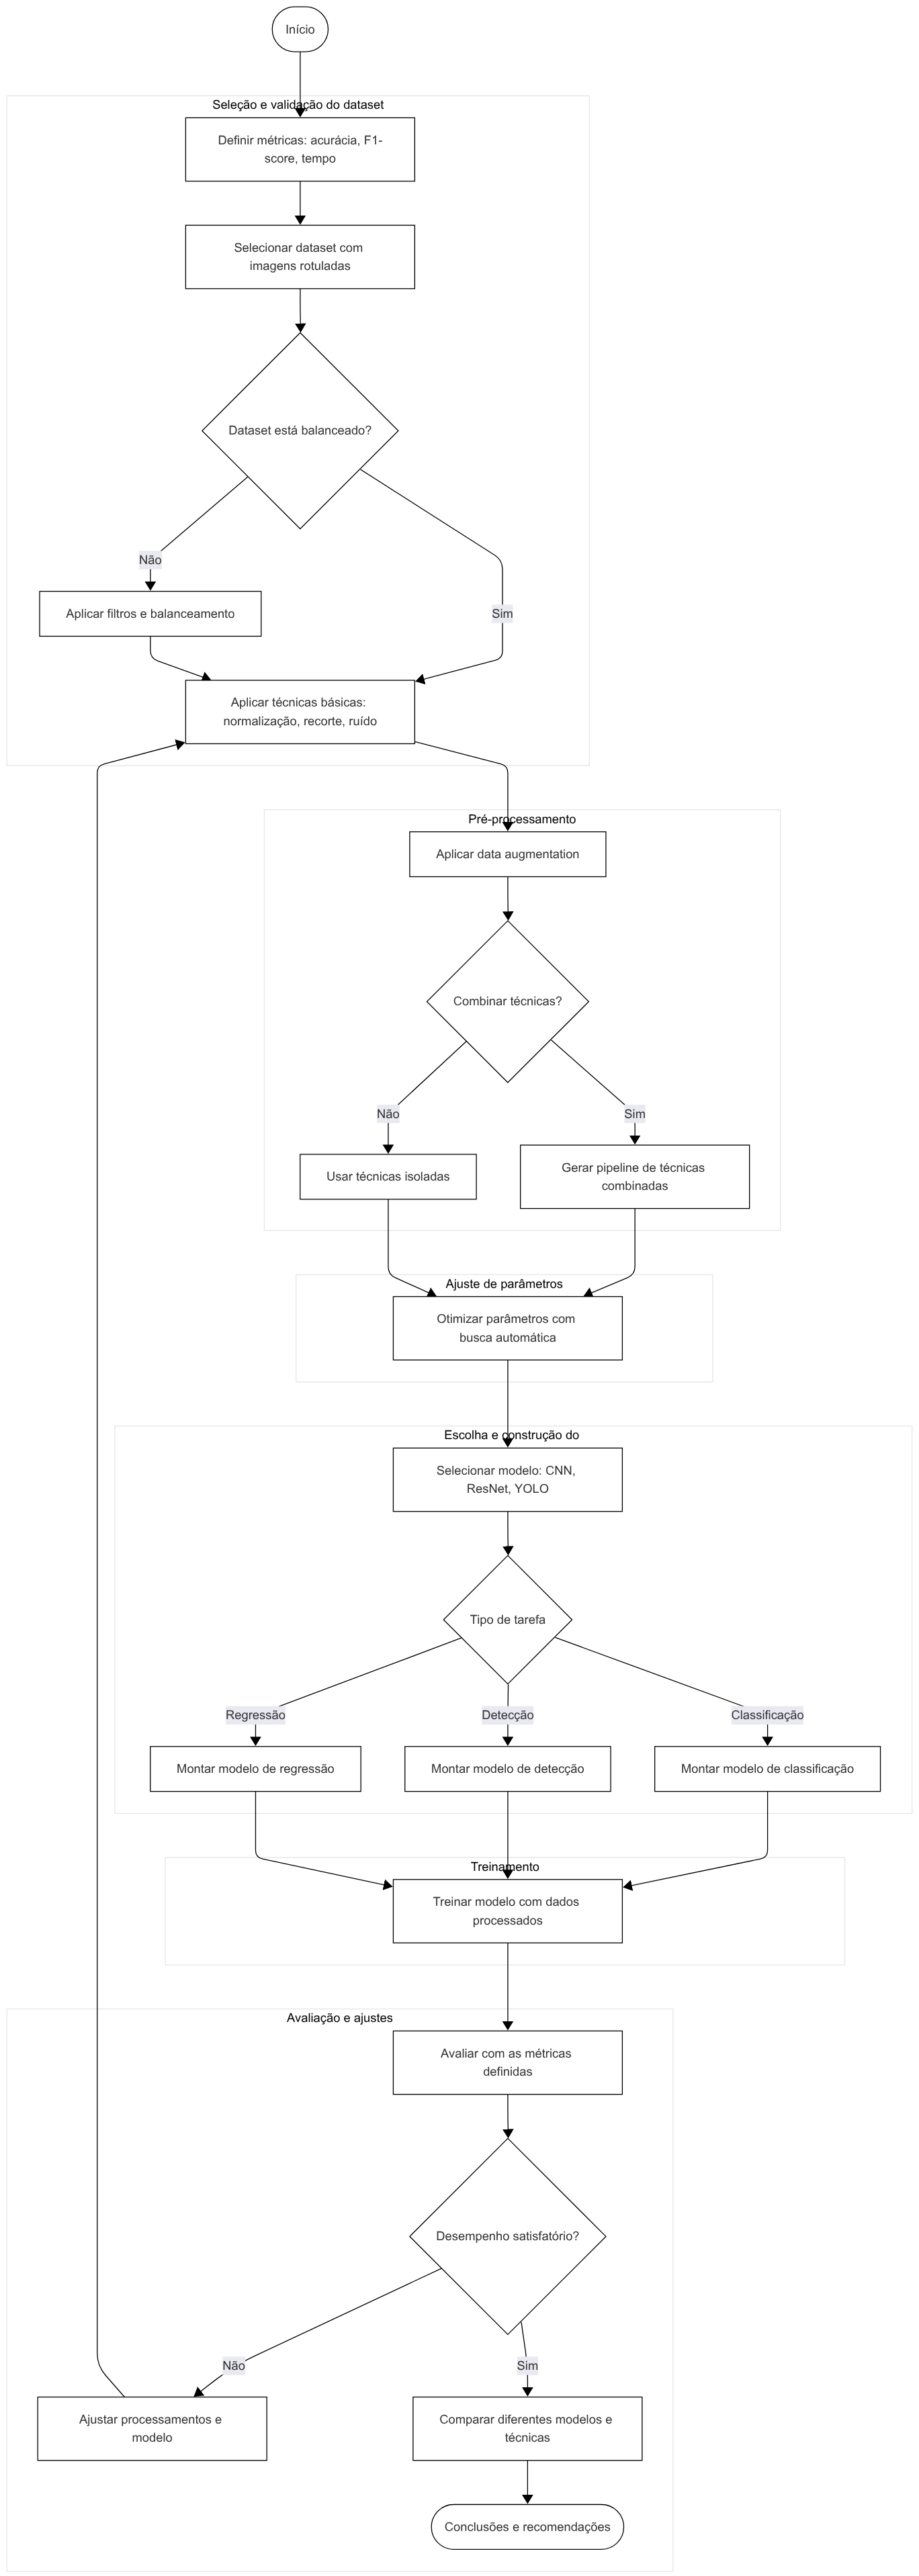
\includegraphics[width=0.5\textwidth]{img/metodologia.png}
    \fonte{Autor.}
\end{figure}

\section{Análise Qualitativa Crítica do Fluxograma}

O fluxograma da metodologia, apresentado na Figura \ref{fig:fluxograma_metodologia}, revela uma arquitetura robusta e pensada para a otimização de processamentos de imagens. Um dos pilares desta estrutura é a natureza iterativa do processo, evidenciada pelos ciclos de "Analisar os resultados" e "Ajustar hiperparâmetros" que retroalimentam a fase de "Pré-processamento". Essa recursividade é crucial, pois permite um refinamento contínuo das técnicas e parâmetros, adaptando-se aos s obtidos a cada iteração. A organização em módulos distintos, como "Construção e treinamento de modelo", "Metodologia de aprimoramento", "Análise de influência" e "Métricas", é outra característica louvável, facilitando a depuração e o aprimoramento localizado de cada componente da metodologia. Essa modularidade assegura que, em caso de falhas ou resultados subótimos, a origem do problema possa ser isolada e corrigida eficientemente, sem comprometer a integridade do sistema como um todo.

Contudo, apesar de sua solidez conceitual, a representação visual do fluxograma em si poderia ser aprimorada para maior clareza. Algumas transições e pontos de decisão, como "Escolheu novo tipo de modelo?" e "Fim da execução dos pré-processamentos?", carecem de detalhes explícitos quanto aos critérios que guiam essas escolhas. A explicitação de limiares ou condições de parada para esses nós de decisão tornaria o fluxograma ainda mais autoexplicativo e replicável. Além disso, a ausência de um rótulo de "Início" formal no primeiro bloco, embora implicitamente compreendido como tal, e a densidade de linhas em certas áreas, podem gerar uma breve confusão inicial para o leitor. Tais observações, no entanto, não diminuem o valor intrínseco da abordagem proposta, que se mantém coerente e alinhada com os objetivos da pesquisa, promovendo um ciclo virtuoso de otimização e aprendizado.

\section{Construção e Treinamento do Modelo}

Esta seção pormenoriza as fases iniciais da metodologia, que envolvem a preparação do ambiente, a aquisição e o tratamento dos dados, bem como a configuração fundamental para o treinamento das arquiteturas de redes neurais que servirão como base para a avaliação dos processamentos de imagem.

\subsection{Início}
O bloco "Início" demarca o ponto de partida formal da execução desta metodologia. Sua função primordial é a de inicializar o ambiente computacional e todos os recursos necessários, garantindo que as ferramentas de software, as bibliotecas de programação e os s de g estejam devidamente configurados e acessíveis. A expectativa é que, ao transitar por este ponto, o sistema esteja plenamente preparado para as operações subsequentes de coleta, tratamento e processamento de dados. A presença deste bloco, embora aparentemente trivial, é crucial para a organização lógica do fluxo de trabalho, servindo como um marco zero que assegura a rastreabilidade e a replicabilidade do experimento.

A dificuldade inerente a esta etapa é, em geral, baixa, confinando-se principalmente à fase de setup inicial do projeto. No cenário de um erro, como a falha na inicialização de bibliotecas ou na alocação de recursos, a ação corretiva imediata seria a verificação das dependências de software, a compatibilidade de versões e a adequação do hardware (por exemplo, disponibilidade de GPUs para aceleração de treinamento). A avaliação do sucesso é intrínseca à própria continuidade do fluxograma: uma transição fluida para o próximo estágio é o indicador de que o "Início" foi bem-sucedido. Este bloco, portanto, alinha-se diretamente ao objetivo geral de desenvolver uma metodologia capaz de comparar, selecionar, combinar e aprimorar técnicas de processamento de imagem, pois estabelece as bases operacionais para todas as etapas subsequentes. Sem essa formalização inicial, a execução do projeto careceria de um ponto de partida definido, comprometendo a sistematicidade proposta.

\subsection{Coletar e tratar os dados de um novo dataset}
A etapa de "Coletar e tratar os dados de um novo dataset" é uma das mais críticas e de maior impacto sobre a qualidade e a confiabilidade dos resultados de qualquer modelo de g. A expectativa é que, nesta fase, os dados brutos -- no contexto deste trabalho, imagens de cadeias de isoladores -- sejam não apenas adquiridos, mas também submetidos a um rigoroso processo de curadoria, limpeza e pré-processamento inicial. Isso pode envolver a padronização de formatos, a remoção de imagens duplicadas ou de baixa qualidade, e, crucialmente, a anotação de falhas para as tarefas de detecção e classificação. Esta etapa é fundamental porque a qualidade, quantidade e diversidade do t impactam diretamente o desempenho e a capacidade de generalização dos modelos de aprendizado de máquina. Sem dados adequados, qualquer processamento subsequente será comprometido. Como mencionado por Shorten et al. (2019) \cite{Shorten2019}, a robustez de um modelo depende intrinsecamente da riqueza de seu conjunto de treinamento.

A dificuldade de execução deste bloco pode ser consideravelmente alta devido à heterogeneidade dos dados, necessidade de anotação manual e desbalanceamento de classes. Datasets para detecção de falhas em isoladores são frequentemente escassos e desbalanceados, com um número muito menor de amostras de falhas do que de isoladores saudáveis. Essa assimetria, conforme He e Garcia (2009) \cite{He2009}, pode levar a modelos enviesados. A anotação manual de imagens, especialmente em grandes volumes ou com defeitos sutis, é um processo demorado e propenso a erros. Se ocorrerem problemas, como a identificação de um t excessivamente pequeno ou desbalanceado, estratégias como aumento de dados (n), que artificialmente expandem o t através de transformações (rotações, espelhamentos, ajustes de brilho/contraste) \cite{Shorten2019}, ou aprendizado semi-supervisionado, que aproveita dados não rotulados, podem ser implementadas. Para o desbalanceamento, a reamostragem (sobreamostragem da classe minoritária ou subamostragem da majoritária) ou o uso de funções de perda focais são abordagens valiosas. O sucesso desta etapa é avaliado tanto pela integridade e organização dos dados resultantes quanto, indiretamente, pelo desempenho inicial razoável dos modelos treinados com esses dados. Este bloco contribui diretamente para o objetivo específico de avaliar a influência do o, uma vez que fornece a base de dados testada sob diversas condições. A garantia de que a metodologia lida com os desafios reais dos s é fundamental para sua aplicabilidade e para que se atinja o objetivo de aprimorar o processamento de imagens.

\subsection{Realizar a validação cruzada do dataset}
O bloco "Realizar a validação cruzada do dataset" é um procedimento metodológico essencial que visa garantir a robustez e a capacidade de generalização dos modelos desenvolvidos. A expectativa é que, ao final desta etapa, o conjunto de dados tenha sido particionado de forma sistemática -- tipicamente utilizando abordagens como a validação cruzada k-fold -- em subconjuntos distintos para treinamento, validação e teste. Essa separação meticulosa é crucial para assegurar que a avaliação do desempenho do modelo seja imparcial e representativa de sua performance em dados não vistos. Ao expor o modelo a diferentes partições dos dados durante o treinamento e a validação, mitiga-se o risco de sobreajuste (g), onde o modelo memoriza o conjunto de treinamento em vez de aprender padrões generalizáveis, como destacado por Goodfellow, Bengio e Courville (2016) \cite{Goodfellow2016}.

A dificuldade de execução desta etapa é geralmente moderada. Erros comuns podem incluir partições mal distribuídas (por exemplo, uma dobra de validação com poucas amostras de uma classe minoritária) ou uma configuração inadequada do número de s. Se a validação cruzada apresentar resultados inconsistentes entre as dobras, a ação corretiva pode envolver a revisão da lógica de divisão dos dados, a implementação de estratégias de estratificação para garantir a representatividade das classes em cada dobra, ou o aumento do número de s para uma avaliação mais abrangente. A avaliação do sucesso é realizada pela consistência no desempenho do modelo em todas as diferentes iterações da validação cruzada; se as métricas de desempenho (como acurácia, precisão, recall) mantêm-se estáveis e satisfatórias em cada dobra, o processo de validação cruzada foi bem-sucedido. Este bloco está intrinsecamente ligado ao objetivo de estabelecer métricas para avaliar a eficácia dos processamentos de imagem, pois a validação cruzada fornece a estrutura necessária para que essas métricas sejam calculadas de maneira confiável e imparcial. Ao garantir uma avaliação fidedigna, a metodologia pode, de fato, comparar e aprimorar as técnicas de processamento de imagem com base em evidências sólidas.

\subsection{Escolheu novo tipo de modelo?}
O bloco de decisão "Escolheu novo tipo de modelo?" representa um ponto estratégico na metodologia que permite a flexibilidade na exploração de diferentes arquiteturas de redes neurais. A expectativa é que esta decisão seja tomada com base em uma análise inicial do desempenho das arquiteturas pré-existentes ou na necessidade de testar novas abordagens que possam se adequar melhor ao problema de detecção e classificação de falhas. Isso pode significar a transição de um modelo de Perceptron (FFN) para uma Convolutional Neural Network (CNN), ou a exploração de variantes específicas dentro dessas categorias. Esta etapa é crucial para o objetivo de analisar o impacto da escolha do modelo de rede neural no desempenho do processamento, visto que, como apontado por Alex (2020) \cite{alex2020}, diferentes tipos de redes neurais possuem princípios de funcionamento e aplicações práticas distintas.

A dificuldade de execução deste bloco é relativamente baixa, pois se trata de uma decisão estratégica. No entanto, uma escolha inadequada pode levar a um ciclo de otimização ineficiente, desperdiçando recursos computacionais e tempo. Se a arquitetura de modelo escolhida não apresentar o desempenho esperado ou não for adequada para o tipo de dados (por exemplo, usar um Perceptron para imagens complexas onde CNNs são mais eficientes), a ação corretiva seria a reavaliação da arquitetura do modelo, considerando suas características intrínsecas e a natureza do problema. A avaliação do sucesso é medida pela capacidade de a nova arquitetura trazer potenciais melhorias no desempenho do sistema ou por fornecer s valiosos sobre a interação entre o tipo de modelo e as técnicas de processamento de imagem. Este bloco contribui diretamente para o alcance do objetivo de analisar o impacto da escolha do modelo de rede neural no desempenho do processamento, pois permite que a metodologia investigue sistematicamente como diferentes modelos afetam a eficácia dos processamentos de imagem, pavimentando o caminho para o aprimoramento contínuo.

\subsection{Retreinar o modelo de rede neural para avaliar os processamentos}
O bloco "Retreinar o modelo de rede neural para avaliar os processamentos" é o cerne do aprendizado e da adaptação do sistema. A expectativa é que, nesta fase, a arquitetura da rede neural previamente selecionada seja re-treinada ou ajustada (d) utilizando os dados que passaram pelas mais recentes iterações de processamento de imagem. O propósito central é que o modelo aprenda a identificar e classificar as falhas nas imagens de isoladores, ajustando seus pesos e s de forma a minimizar a função de custo e otimizar as métricas de desempenho. Como explicam Braga e Silva (2011) \cite{Braga2011}, o treinamento é onde o neurônio artificial aprende a associar entradas a saídas desejadas. A importância deste bloco é vital, pois os modelos de redes neurais não são apenas as ferramentas para a detecção de falhas, mas também os avaliadores do impacto dos diferentes processamentos de imagem.

A dificuldade de execução pode ser alta, dada a complexidade do treinamento de redes neurais. Desafios incluem a otimização de hiperparâmetros (como taxa de aprendizado, tamanho do h, número de épocas), o gerenciamento de recursos computacionais (tempo de processamento, memória de GPU) e a mitigação do sobreajuste (g). Se o modelo não convergir, apresentar baixo desempenho ou superajuste, as ações corretivas podem envolver: a modificação dos hiperparâmetros do treinamento, a escolha de otimizadores mais adequados (como Adam \cite{Kingma2014} ou RMSProp \cite{Tieleman2012}, que ajustam a taxa de aprendizado), a aplicação de técnicas de regularização (como t), a expansão do t (se houver escassez persistente) ou a revisão da própria arquitetura da rede neural. A avaliação do sucesso é multifacetada: a diminuição progressiva da função de custo durante o treinamento e, crucialmente, o aumento das métricas de desempenho (acurácia, precisão, recall, F1-score) nos conjuntos de validação e teste, indicam que o modelo está aprendendo de forma eficaz. Este bloco alinha-se diretamente ao objetivo de construir modelos de redes neurais destinados à avaliação do desempenho das técnicas de processamento de imagem, pois é através do treinamento que esses modelos adquirem a capacidade de realizar tal avaliação. Ao refinar continuamente esses modelos, a metodologia garante que a avaliação dos processamentos de imagem seja feita com a maior precisão possível, contribuindo para o aprimoramento geral do sistema.

\section{Metodologia de Aprimoramento}

Esta seção aprofunda as abordagens sistemáticas para otimizar as imagens, com foco na aplicação e combinação de técnicas específicas.

\subsection{Pré-processamento}
O bloco de "Pré-processamento" é uma fase fundamental onde as imagens são preparadas para maximizar a eficácia dos modelos de rede neural. A expectativa é que esta etapa envolva a aplicação de diversas técnicas de processamento de imagem, como a normalização (padronização dos valores de pixels para escalas como [0,1] ou Z-score) \cite{Sharma2024}, o redimensionamento e recorte (ajustando imagens para as dimensões de entrada do modelo e extraindo regiões de interesse) \cite{Sharma2024}, a redução de ruído (eliminando interferências com filtros como mediana ou CNNs especializadas) \cite{Sharma2024}, o ajuste de contraste e brilho (melhorando a visibilidade de características importantes) \cite{Sharma2024}, o aumento de nitidez (realçando bordas e detalhes finos) \cite{Sharma2024}, a conversão de espaço de cores (adaptando a representação das cores às necessidades da tarefa) \cite{Sharma2024}, a restauração e desembaçamento (recuperando imagens degradadas) \cite{Sharma2024}, e a detecção de bordas (identificando limites e formas) \cite{Sharma2024}. Essas operações são cruciais porque, como afirmado por Sharma et al. (2024) \cite{Sharma2024}, elas "melhoram a qualidade das imagens, mas também garantem que os modelos sejam mais robustos e capazes de generalizar em diferentes condições".

A dificuldade de execução pode variar de média a alta, dependendo da complexidade das técnicas e da necessidade de ajuste fino dos seus parâmetros. Um erro comum é a aplicação excessiva de pré-processamento, que, em vez de aprimorar, pode degradar o desempenho do modelo ao remover informações úteis, como alertado por Öztürk e Akdemir (2018) \cite{Ozturk2018} e Rodrigues, Naldi e Mari (2020) \cite{Rodrigues2020}. Se o desempenho do modelo piorar após um pré-processamento, a ação corretiva seria revisar a técnica aplicada, seus parâmetros ou até mesmo revertê-la, buscando um equilíbrio. A avaliação do sucesso é dual: primeiramente, por uma análise visual qualitativa das imagens processadas (elas parecem mais claras, com características mais proeminentes?). Em segundo lugar, e mais importante, pelo impacto quantitativo no desempenho do modelo de rede neural (acurácia, precisão, recall, F1-score e mAP para detecção de objetos). Este bloco é central para o objetivo geral de aprimorar técnicas de processamento de imagem, pois é aqui que as transformações diretas nas imagens são testadas e validadas, contribuindo para que a metodologia identifique as estratégias mais eficazes para aprimorar a detecção de falhas.

\subsection{Fim da execução dos pré-processamentos?}
O bloco de decisão "Fim da execução dos pré-processamentos?" atua como um mecanismo de controle e de iteração dentro do fluxo da metodologia, estabelecendo um ponto de verificação para a fase de aprimoramento das imagens. A expectativa é que esta decisão seja tomada após um número predefinido de iterações, ou quando as melhorias nas métricas de desempenho se tornarem marginais. O propósito deste bloco é assegurar que a exploração das diferentes técnicas de pré-processamento -- tanto individualmente quanto em combinações -- seja suficientemente exaustiva, mas sem incorrer em um gasto computacional desnecessário. Ele direciona o fluxo, decidindo se o processo de teste de pré-processamentos deve continuar (retornando ao estágio anterior) ou se os resultados atuais já são satisfatórios para prosseguir para a análise e otimização.

A dificuldade de execução desta etapa é baixa, sendo essencialmente um ponto lógico de bifurcação. No entanto, uma decisão prematura pode resultar em uma otimização incompleta, negligenciando combinações ou ajustes de parâmetros potencialmente mais eficazes. Se os resultados obtidos até o momento não demonstrarem um aprimoramento significativo, a ação corretiva seria revisitar o critério de parada ou explorar novas configurações e combinações de pré-processamentos que ainda não foram testadas. A avaliação do sucesso reside na abrangência da exploração das possibilidades de pré-processamento e na garantia de que as melhores configurações foram investigadas. Este bloco é crucial para o objetivo de desenvolver uma metodologia para o aprimoramento dos processamentos de imagem, pois ao gerenciar o ciclo de testes e refinamento, ele assegura que a metodologia não pare de buscar aprimoramento antes de esgotar as opções razoáveis, contribuindo para a robustez da solução final.

\subsection{Ajuste automático de parâmetros}
O bloco "Ajuste automático de parâmetros" representa um avanço significativo na eficiência da metodologia, substituindo a tediosa e muitas vezes inviável otimização manual. A expectativa é que, nesta fase, algoritmos de otimização automatizada sejam empregados para encontrar os valores ideais para os parâmetros das técnicas de processamento de imagem que estão sendo testadas. Isso pode incluir, por exemplo, a intensidade de um filtro de desfoque, o limiar de um ajuste de contraste, ou os s de uma técnica de redução de ruído. O propósito fundamental deste bloco é otimizar os resultados dos processamentos sem exigir extensa intervenção manual, como destacado na proposta da metodologia. A automação não apenas acelera o processo, mas também tem o potencial de descobrir configurações de parâmetros que seriam difíceis de identificar heuristicamente.

A dificuldade de execução pode ser alta, pois envolve a seleção e implementação de algoritmos de otimização (por exemplo, algoritmos genéticos, otimização por enxame de partículas, otimização Bayesiana) e a definição de um espaço de busca adequado para os parâmetros. Um erro comum é a convergência para ótimos locais em vez do ótimo global, ou um tempo computacional proibitivo para a busca. Se o ajuste automático não encontrar parâmetros que resultem em melhorias significativas, as ações corretivas podem incluir: a modificação do algoritmo de otimização, a redefinição das faixas de valores para os parâmetros, ou a incorporação de critérios de parada mais sofisticados. A avaliação do sucesso é diretamente quantitativa: a melhoria mensurável nas métricas de desempenho do modelo de rede neural após a aplicação dos parâmetros otimizados automaticamente indica que o processo foi bem-sucedido. Este bloco está diretamente ligado ao objetivo específico de criar um método de ajuste automático de parâmetros dos processamentos de imagem, sendo um pilar central para o aprimoramento contínuo e eficiente das técnicas, e, por consequência, para o objetivo geral da metodologia.

\subsection{Combinação de abordagens unitárias}
O bloco "Combinação de abordagens unitárias" é uma etapa inovadora e potencialmente transformadora na metodologia, focando na sinergia entre diferentes técnicas de processamento de imagem. A expectativa é que, nesta fase, diversas operações de processamento, previamente testadas individualmente como "processamentos unitários", sejam sequenciadas ou combinadas de maneiras estratégicas para gerar um efeito cumulativo que transcenda o impacto de cada técnica isolada. Por exemplo, uma imagem pode ser primeiramente submetida à redução de ruído, seguida por um ajuste de contraste e, finalmente, por um aumento de nitidez. O propósito é explorar o potencial de melhoria que reside na interação entre diferentes processamentos, realçando aspectos complementares da imagem e otimizando a qualidade final para a detecção de falhas. A proposta baseia-se na ideia de que a combinação de técnicas pode resultar em "melhorias significativas no desempenho dos sistemas de diagnóstico".

A dificuldade de execução pode ser de média a alta, principalmente devido à explosão combinatória de possibilidades (a ordem e a seleção das técnicas importam) e à necessidade de identificar as sequências mais eficazes. Um erro comum é a criação de combinações que introduzem artefatos ou degradam a imagem, em vez de aprimorá-la. Se as combinações não funcionarem, as ações corretivas podem incluir: a exploração de diferentes ordens de aplicação, a limitação do número de técnicas em uma sequência, ou o uso de algoritmos de busca heurística para navegar no espaço de combinações. A avaliação do sucesso é realizada pela melhoria nas métricas de desempenho da rede neural (acurácia, precisão, recall, F1-score) quando as imagens processadas pela combinação são utilizadas como entrada. Este bloco está diretamente ligado ao objetivo de desenvolver uma metodologia para o aprimoramento dos processamentos de imagem por meio da combinação de diferentes abordagens unitárias. Ao permitir a investigação sistemática dessas combinações, a metodologia visa descobrir sequências ótimas que levam a um desempenho superior na detecção e classificação de falhas, contribuindo substancialmente para o objetivo geral do trabalho.

\section{Análise de Influência}

Esta seção detalha a investigação sobre como diferentes fatores, como os dados de entrada e o tipo de modelo, afetam o desempenho do sistema, fornecendo s valiosos para a otimização.

\subsection{Analisar a influência do dataset}
O bloco "Analisar a influência do dataset" é uma etapa crucial que visa aprofundar a compreensão sobre como as características intrínsecas dos conjuntos de dados de imagens afetam diretamente a eficácia das técnicas de processamento e, consequentemente, o desempenho dos modelos de rede neural na detecção de falhas. A expectativa é que, nesta fase, sejam conduzidos experimentos sistemáticos utilizando diferentes s (ou variações do mesmo t, como subconjuntos com distintas distribuições de falhas ou condições de iluminação), e os resultados sejam comparados exaustivamente. O propósito é identificar como fatores como o tamanho do dataset, a sua diversidade, a presença de ruídos específicos ou o grau de desbalanceamento entre as classes de falha e não falha influenciam a performance.

A dificuldade de execução desta etapa é de média a alta, pois exige a aquisição e o pré-processamento de múltiplos s, a execução de experimentos comparativos e uma análise estatística rigorosa dos resultados. Um erro comum é tirar conclusões precipitadas de um único t. Se a análise não for conclusiva, ou seja, se não houver um padrão claro de como o t influencia o desempenho, as ações corretivas podem incluir a coleta de dados adicionais que representem uma gama mais ampla de condições, a refinamento das métricas de avaliação para capturar nuances específicas do desempenho ou a utilização de testes de hipótese estatística para validar as observações. A avaliação do sucesso é confirmada pela identificação de correlações claras e s sobre como as propriedades do t afetam a performance do sistema. Este bloco contribui diretamente para o objetivo específico de avaliar a influência do o, permitindo que a metodologia proponha soluções mais adaptáveis e robustas, capazes de lidar com a variabilidade do mundo real.

\subsection{Analisar a influência do modelo}
O bloco "Analisar a influência do modelo" é uma vertente de pesquisa crucial que investiga a interdependência entre a escolha da arquitetura da rede neural e a eficácia das técnicas de processamento de imagem. A expectativa é que, nesta etapa, diferentes tipos de modelos de redes neurais, como redes convolucionais (CNNs) e redes Perceptron (FFNs), sejam testados com as mesmas imagens processadas por diversas técnicas. O objetivo é compreender como a estrutura e as capacidades inerentes de cada modelo interagem com as características realçadas ou modificadas pelos processamentos de imagem. Essa análise é fundamental, pois, como destacado na proposta, "diferentes modelos podem gerar resultados distintos para um mesmo processamento". Identificar qual modelo se beneficia mais de um tipo específico de pré-processamento ou combinação é essencial para a otimização global da metodologia.

A dificuldade de execução desta etapa é de média a alta, demandando a implementação e o treinamento de múltiplas arquiteturas de redes neurais, cada uma otimizada em seus próprios hiperparâmetros para garantir uma comparação justa. Um erro comum é atribuir variações de desempenho exclusivamente ao processamento de imagem, ignorando a capacidade de extração de características do modelo. Se a análise não for conclusiva, as ações corretivas podem envolver: a inclusão de mais arquiteturas de modelos para uma exploração mais ampla, o ajuste fino mais rigoroso dos hiperparâmetros de cada modelo ou a utilização de técnicas de interpretabilidade de IA (XAI) para visualizar quais características o modelo está aprendendo a partir das imagens processadas. A avaliação do sucesso é aferida pela identificação de padrões claros de desempenho que demonstrem como certas combinações de modelo e pré-processamento resultam em resultados superiores. Este bloco está diretamente ligado ao objetivo de analisar o impacto da escolha do modelo de rede neural no desempenho do processamento. Ao elucidar essas interações, a metodologia pode recomendar as combinações mais eficazes, contribuindo significativamente para o aprimoramento geral da detecção de falhas.

\section{Métricas}

Esta seção define as ferramentas quantitativas essenciais para avaliar o sucesso das intervenções na metodologia, garantindo uma análise objetiva do desempenho.

\subsection{Tempo de processamento}
O bloco "Tempo de processamento" foca na avaliação da eficiência computacional das diferentes técnicas e sequências de processamento de imagem, bem como da inferência dos modelos de rede neural. A expectativa é que sejam coletadas medições precisas do tempo decorrido para cada operação e para o e completo de detecção e classificação de falhas. O propósito deste bloco é tão crítico quanto a acurácia, especialmente em aplicações industriais onde a resposta em tempo real é um requisito imperativo, como na inspeção de linhas de transmissão por VANTs. Como destacado por Peng et al. (2023) \cite{Peng2023}, a eficiência computacional é uma consideração primária para modelos como YOLOv5 e YOLOv7 em cenários de inspeção.

A dificuldade de execução desta medição é geralmente baixa, utilizando s e g de software. No entanto, variações no ambiente de execução (hardware, carga do sistema) podem introduzir ruído nas medições. Se o tempo de processamento for considerado excessivamente alto para a aplicação-alvo, as ações corretivas podem incluir: a otimização de algoritmos, a exploração de implementações mais eficientes (por exemplo, usando GPUs ou s otimizados), a redução da complexidade dos modelos ou a seleção de técnicas de processamento mais leves. A avaliação do sucesso é determinada pela capacidade de atingir ou exceder os requisitos de tempo para a aplicação prática. Este bloco alinha-se diretamente ao objetivo de estabelecer métricas para avaliar a eficácia dos processamentos de imagem, considerando aspectos como ... tempo de processamento. Ao incorporar a dimensão temporal, a metodologia garante que as soluções propostas não sejam apenas precisas, mas também viáveis para implantação em cenários reais, consolidando seu valor prático.

\subsection{Métricas de eficácia de modelos de IA (acurácia, precisão, recall, f1-score)}
O bloco "Métricas de eficácia de modelos de IA (acurácia, precisão, recall, f1-score)" é a espinha dorsal da avaliação quantitativa do desempenho do sistema de detecção e classificação de falhas. A expectativa é que, nesta fase, sejam calculadas e analisadas criticamente um conjunto de métricas robustas, que ofereçam uma visão multifacetada da performance do modelo. Além da acurácia (proporção de previsões corretas), que, embora útil, pode ser enganosa em s desbalanceados \cite{He2009}, serão avaliadas a precisão (proporção de verdadeiros positivos entre todas as previsões positivas), o recall (sensibilidade) (proporção de verdadeiros positivos entre todas as amostras positivas reais) e o F1-score (média harmônica entre precisão e recall, ideal para cenários desbalanceados). Para tarefas de detecção de objetos, a mAP (média da precisão média) será empregada, e a AUC-ROC também será considerada para avaliar a capacidade discriminativa do modelo. A matriz de confusão fornecerá uma visão detalhada dos erros. O propósito dessas métricas é fornecer uma avaliação compreensiva e imparcial do quão bem o modelo está detectando e classificando as falhas, especialmente considerando que falsos negativos (falhas não detectadas) podem ter consequências graves.

A dificuldade de execução é moderada, residindo mais na interpretação correta das métricas em diferentes contextos de problema, especialmente em face de s desbalanceados. Se as métricas forem insatisfatórias (por exemplo, recall baixo para a classe de falhas), as ações corretivas podem envolver: a revisão e otimização dos pré-processamentos de imagem, o ajuste fino dos hiperparâmetros do modelo de rede neural, a reaplicação de técnicas para lidar com desbalanceamento de dados (reamostragem, perda focal) ou, em última instância, a revisão da arquitetura do modelo. A avaliação do sucesso é medida pela obtenção de valores elevados e balanceados nessas métricas, indicando um modelo confiável e eficaz. Este bloco é central para o objetivo de estabelecer métricas para avaliar a eficácia dos processamentos de imagem, pois são essas métricas que permitem a quantificação e comparação rigorosa do impacto de cada intervenção na metodologia, assegurando que o aprimoramento seja validado de forma científica.

\section{Avaliação e Conclusão}

Esta seção finaliza a metodologia, abordando a consolidação dos resultados, a autoavaliação do processo e as diretrizes para futuras explorações.

\subsection{Coletar resultados}
O bloco "Coletar resultados" é a etapa crucial de agregação de todas as informações de desempenho geradas ao longo da metodologia. A expectativa é que, ao final desta fase, tenha-se uma base de dados organizada e completa contendo as métricas de eficácia (acurácia, precisão, recall, F1-score, mAP, AUC-ROC) e os tempos de processamento para cada combinação de técnica de pré-processamento, parâmetros e modelo de rede neural testada. O propósito primordial deste bloco é fornecer a base empírica necessária para a análise comparativa das diferentes abordagens, permitindo identificar quais estratégias são mais promissoras e por quê. É o momento de consolidar os dados brutos de desempenho em um formato que facilite a interpretação e a tomada de decisões subsequentes.

A dificuldade de execução desta etapa é relativamente baixa, assumindo que um sistema de registro de experimentos (por exemplo, uso de s, bancos de dados ou planilhas estruturadas) tenha sido implementado desde o início. No entanto, um erro comum é a falha em registrar todas as variáveis relevantes ou a inconsistência no formato dos dados. Se os resultados estiverem incompletos, inconsistentes ou difíceis de interpretar, a ação corretiva seria a revisão dos protocolos de registro de dados e a padronização das informações coletadas em todas as execuções. A avaliação do sucesso é confirmada pela disponibilidade de um conjunto de dados de desempenho compreensível e completo, pronto para ser submetido à análise. Este bloco é fundamental para o objetivo geral de comparar, selecionar, combinar e aprimorar técnicas de processamento de imagem, pois a capacidade de realizar uma análise eficaz depende diretamente da qualidade e organização dos dados coletados. Sem uma coleta sistemática, as etapas de análise e validação seriam comprometidas.

\subsection{Analisar os resultados}
O bloco "Analisar os resultados" representa a fase de interpretação crítica e síntese dos dados de desempenho coletados. A expectativa é que, utilizando técnicas de análise de dados (estatísticas descritivas, gráficos comparativos, testes de significância), sejam identificados padrões claros de desempenho, tendências, e as combinações mais eficazes entre processamentos de imagem, parâmetros e modelos de rede neural. O propósito deste bloco é extrair s sobre o que funciona, o que não funciona e por quê, informando as próximas iterações do ciclo de otimização ou as conclusões finais da pesquisa. É aqui que se determina, por exemplo, se um tipo de pré-processamento específico (como a equalização de histograma) melhorou consistentemente o desempenho de uma CNN em s com baixa iluminação.

A dificuldade de execução desta etapa é de média a alta, exigindo sólidas habilidades analíticas, conhecimento em estatística e ferramentas de visualização de dados. Um erro comum é a interpretação enviesada dos resultados ou a incapacidade de identificar as causas-raiz das variações de desempenho. Se a análise não fornecer s claros ou se as conclusões forem ambíguas, as ações corretivas podem incluir: a redefinição das perguntas de pesquisa, a aplicação de técnicas de análise mais avançadas (como ANOVA, regressão), ou a exploração de visualizações de dados alternativas para revelar padrões ocultos. A avaliação do sucesso é dada pela geração de conclusões claras, s e a capacidade de explicar as variações de desempenho de forma consistente. Este bloco é crucial para o objetivo geral de comparar, selecionar, combinar e aprimorar técnicas de processamento de imagem, pois é através de uma análise rigorosa que a metodologia pode discernir as abordagens mais eficazes, garantindo que o aprimoramento seja baseado em evidências empíricas sólidas.

\subsection{Comprovou o aprimoramento?}
O bloco de decisão "Comprovou o aprimoramento?" serve como um ponto de validação crítico na metodologia, determinando se os esforços de otimização resultaram em melhorias significativas e mensuráveis no desempenho do sistema. A expectativa é que esta decisão seja tomada com base em critérios pré-definidos de sucesso, geralmente quantificados pelas métricas de eficácia (acurácia, F1-score, mAP) e/ou pelo tempo de processamento. Por exemplo, pode-se estabelecer um limiar de 2\% de aumento no F1-score como critério para considerar o aprimoramento comprovado. Se o aprimoramento for comprovado, o processo avança para a conclusão e documentação; caso contrário, ele retorna ao bloco de "Ajustar hiperparâmetros" para uma nova iteração de refinamento.

A dificuldade de execução é baixa, pois é uma decisão lógica baseada em dados objetivos. No entanto, é fundamental que os critérios de sucesso sejam bem definidos e realistas para evitar ciclos de otimização infinitos ou a conclusão prematura. Se o aprimoramento não for comprovado apesar de múltiplas iterações de ajuste, as ações corretivas podem envolver: a revisão mais profunda da arquitetura do modelo, a exploração de técnicas de processamento radicalmente diferentes, ou a reavaliação da própria viabilidade de aprimoramento além de um certo ponto para o problema em questão. A avaliação do sucesso reside na atingir as metas de desempenho estabelecidas, indicando que a metodologia foi capaz de otimizar efetivamente o sistema. Este bloco está diretamente ligado ao objetivo de desenvolver uma metodologia capaz de comparar, selecionar, combinar e aprimorar técnicas de processamento de imagem, pois atua como a última validação antes de se considerar o objetivo alcançado. Ele garante que o trabalho não apenas execute processos, mas que esses processos culminem em melhorias reais e verificáveis.

\subsection{Conclusão e documentação}
O bloco "Conclusão e documentação" representa a fase final da metodologia, onde todo o conhecimento adquirido e os resultados obtidos são consolidados e formalizados. A expectativa é que esta etapa culmine na redação de um relatório completo ou artigo acadêmico, que sintetize os principais achados do estudo, conforme a seção 6.1 do documento de referência. Isso inclui a apresentação detalhada das técnicas de processamento de imagem aprimoradas, as combinações mais eficazes, o impacto da escolha do modelo e do t, e as métricas de desempenho alcançadas. Além disso, é crucial discutir as limitações e os desafios encontrados durante a pesquisa, como indicado na seção 6.2, e apresentar sugestões para pesquisas futuras, conforme a seção 6.3, que podem expandir o escopo do trabalho. A documentação deve ser suficientemente detalhada para permitir a replicabilidade dos experimentos e a continuidade da pesquisa por outros investigadores.

A dificuldade de execução desta etapa é moderada, exigindo clareza na escrita, capacidade de síntese e rigor acadêmico. Um erro comum é a falta de detalhe técnico na descrição da metodologia ou a interpretação inadequada dos resultados. Se a documentação for inadequada ou as conclusões não forem bem fundamentadas, as ações corretivas envolvem a revisão e o aprofundamento do texto, buscando maior precisão e clareza. A avaliação do sucesso é medida pela completude, clareza e coerência da documentação produzida, e pela sua capacidade de transmitir os s e as contribuições do trabalho de forma eficaz. Este bloco consolida o cumprimento do objetivo geral de desenvolver uma metodologia capaz de comparar, selecionar, combinar e aprimorar técnicas de processamento de imagem. A formalização e a disseminação do conhecimento gerado garantem que a metodologia não apenas atinja seus objetivos práticos, mas também contribua para o avanço da área de processamento de imagens e inteligência artificial aplicada à detecção de falhas.

\section{Ajuste de Hiperparâmetros}

\subsection{Ajustar hiperparâmetros}
O bloco "Ajustar hiperparâmetros" é uma etapa iterativa e crucial no ciclo de otimização da metodologia, operando como um mecanismo de refinamento do desempenho dos modelos de rede neural. A expectativa é que, nesta fase, os valores dos hiperparâmetros que governam o comportamento do modelo sejam sistematicamente modificados e retestados. Isso inclui elementos como a taxa de aprendizado, o número de camadas ocultas da rede, o número de neurônios por camada, o tamanho do lote (e), as funções de ativação (ReLU \cite{Agarap2018}, Sigmoid \cite{Langer2020}, Softmax \cite{Gao2017}) e os otimizadores (Gradiente Descendente, Adam \cite{Kingma2014}, RMSProp \cite{Tieleman2012}). O propósito central é buscar a configuração ideal que permita ao modelo aprender de forma mais eficiente e generalizar melhor para dados não vistos, impactando diretamente o desempenho na avaliação dos processamentos de imagem. A otimização de hiperparâmetros é, frequentemente, um fator determinante para o sucesso de modelos de g.

A dificuldade de execução desta etapa pode ser consideravelmente alta, dada a natureza empírica e a complexidade do espaço de busca dos hiperparâmetros. Isso é um processo que pode consumir muitos recursos computacionais. Um erro comum é a escolha arbitrária de valores ou a estagnação em um ótimo local, resultando em subotimização. Se o ajuste não resultar em melhorias significativas ou se o desempenho do modelo piorar, as ações corretivas podem envolver: a utilização de estratégias de busca mais avançadas (como h, h, ou otimização Bayesiana para explorar o espaço de hiperparâmetros de forma mais inteligente), a implementação de técnicas de regularização (como t ou g para prevenir o sobreajuste), ou a revisão da própria função de custo utilizada. A avaliação do sucesso é medida pela melhoria quantificável nas métricas de desempenho do modelo no conjunto de validação após a aplicação dos novos hiperparâmetros. Este bloco contribui diretamente para o objetivo de construir modelos de redes neurais e analisar o impacto da escolha do modelo, pois o ajuste de hiperparâmetros é parte integrante do desenvolvimento e da otimização desses modelos. Ao refinar continuamente os modelos através deste processo, a metodologia garante que a avaliação dos processamentos de imagem seja conduzida por avaliadores com desempenho máximo, contribuindo para o aprimoramento geral do sistema.